\documentclass[aspectratio=169,11pt]{beamer}

\makeatletter
\input{../../templates/dune-professional/beamerthemeDUNEProfessional.sty}
\makeatother
\DuneUseWhite
\usetikzlibrary{plotmarks}

\title{Presentation title}
\subtitle{State the audience outcome in one clear sentence}
\author{Presentation author}
\date{Meeting or event -- \today}
\hypersetup{colorlinks=true,urlcolor=DuneInfo,linkcolor=DuneInfo}

\begin{document}

\begin{frame}[plain]
  \titlepage
\end{frame}

\begin{frame}{Tell people the answer first}
  \DuneBigStatement{THE RESULT}
    {Make one claim the evidence supports.}
    {Say what changed, why it matters, and what remains uncertain.}
  \vspace{5mm}
  Name the person who acts next and the result they need to produce.
\end{frame}

\begin{frame}{Compare conditions on the same scale}
  \centering
  \begin{tikzpicture}[x=1.65cm,y=0.48cm,font=\small]
    % Illustrative coordinates only; no measured performance is claimed.
    \draw[DuneTextMuted] (0,0) -- (4.6,0);
    \draw[DuneTextMuted] (0,0) -- (0,6.5);
    \foreach \x in {0,1,2,3,4} {
      \draw[DuneTextMuted] (\x,0) -- (\x,-0.12)
        node[below,text=DuneText] {\x};
    }
    \foreach \y in {0,2,4,6} {
      \draw[DuneTextMuted] (0,\y) -- (-0.06,\y)
        node[left,text=DuneText] {\y};
    }
    \node[below,text=DuneText] at (2,-0.75) {Time (s)};
    \node[above right,text=DuneText] at (0,6.6) {Response (arbitrary units)};
    \draw[DuneText,line width=1pt] plot[mark=*,mark size=1.7pt]
      coordinates {(0,1) (1,2) (2,3) (3,4) (4,5)};
    \draw[DuneTextMuted,dashed,line width=1pt] plot[mark=square*,mark size=1.7pt]
      coordinates {(0,1) (1,1.5) (2,2) (3,2.5) (4,3)};
    \node[right,text=DuneText] at (4.1,5) {Condition A};
    \node[right,text=DuneTextMuted] at (4.1,3) {Condition B};
  \end{tikzpicture}

  \vspace{3mm}
  {\small Illustrative data: two constructed series demonstrate shared axes,
  direct labels, and distinct marks. Replace with sourced measurements.\par}
\end{frame}

\begin{frame}{Label each relationship where it appears}
  \centering
  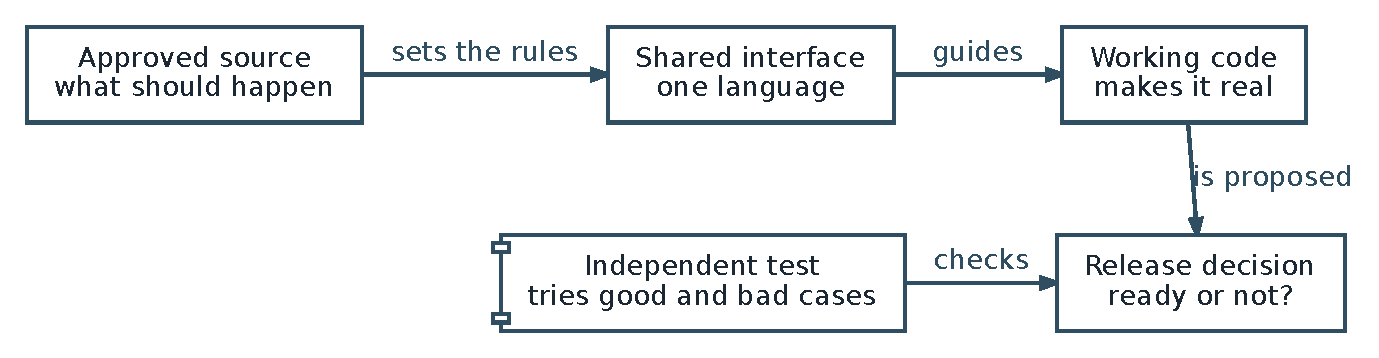
\includegraphics[width=0.91\textwidth,height=0.61\textheight,keepaspectratio]{diagrams/system-context.pdf}

  \vspace{2mm}
  \DuneDiagramCaption{Illustrative release process: source requirements guide
  the code; an independent test informs the release decision. This is not an
  installed system or an agreed assignment of responsibility.}
\end{frame}

\begin{frame}{Keep the evidence and its limits together}
  \begin{columns}[T,onlytextwidth]
    \begin{column}{0.47\textwidth}
      \textbf{What the evidence supports}\par\medskip
      Give the observation, units, source, and conditions needed to read it.
    \end{column}
    \begin{column}{0.47\textwidth}
      \textbf{What remains open}\par\medskip
      State the uncertainty and the check that could change the conclusion.
    \end{column}
  \end{columns}
  \vspace{8mm}
  \textbf{Next action}\par\medskip
  Name the person, the action, and the result that will close the question.
\end{frame}

\end{document}
